%!TEX root = ../template.tex
%%%%%%%%%%%%%%%%%%%%%%%%%%%%%%%%%%%%%%%%%%%%%%%%%%%%%%%%%%%%%%%%%%%%
%% chapter4.tex
%% NOVA thesis document file
%%
%% Chapter with lots of dummy text
%%%%%%%%%%%%%%%%%%%%%%%%%%%%%%%%%%%%%%%%%%%%%%%%%%%%%%%%%%%%%%%%%%%%
\chapter{Elaboration Plan}
\label{cha:elaboration_plan}

This chapter presents the work plan for the elaboration phase of this dissertation. First we summarise the planned tasks as well as their planned time frames all gathered in a Gantt chart presented in section \ref{sec:workplan}. Then, in section \ref{sec:workplan_details} the tasks are described in better detail and more in depth as well as referring the relevant related dependencies and risk-management options.

\section{Work Plan}
\label{sec:workplan}

This section presents the work plan and given timeline of tasks, with start and finish predictions. This estimated times already contain a certain margin to allow for some unforeseen events and complications to the planned work. Figure \ref{fig:work_plan} shows 11 main tasks that are divided in subtasks for a better discrimination and a better detail of the task.

\begin{figure}[htbp]
	\centerline{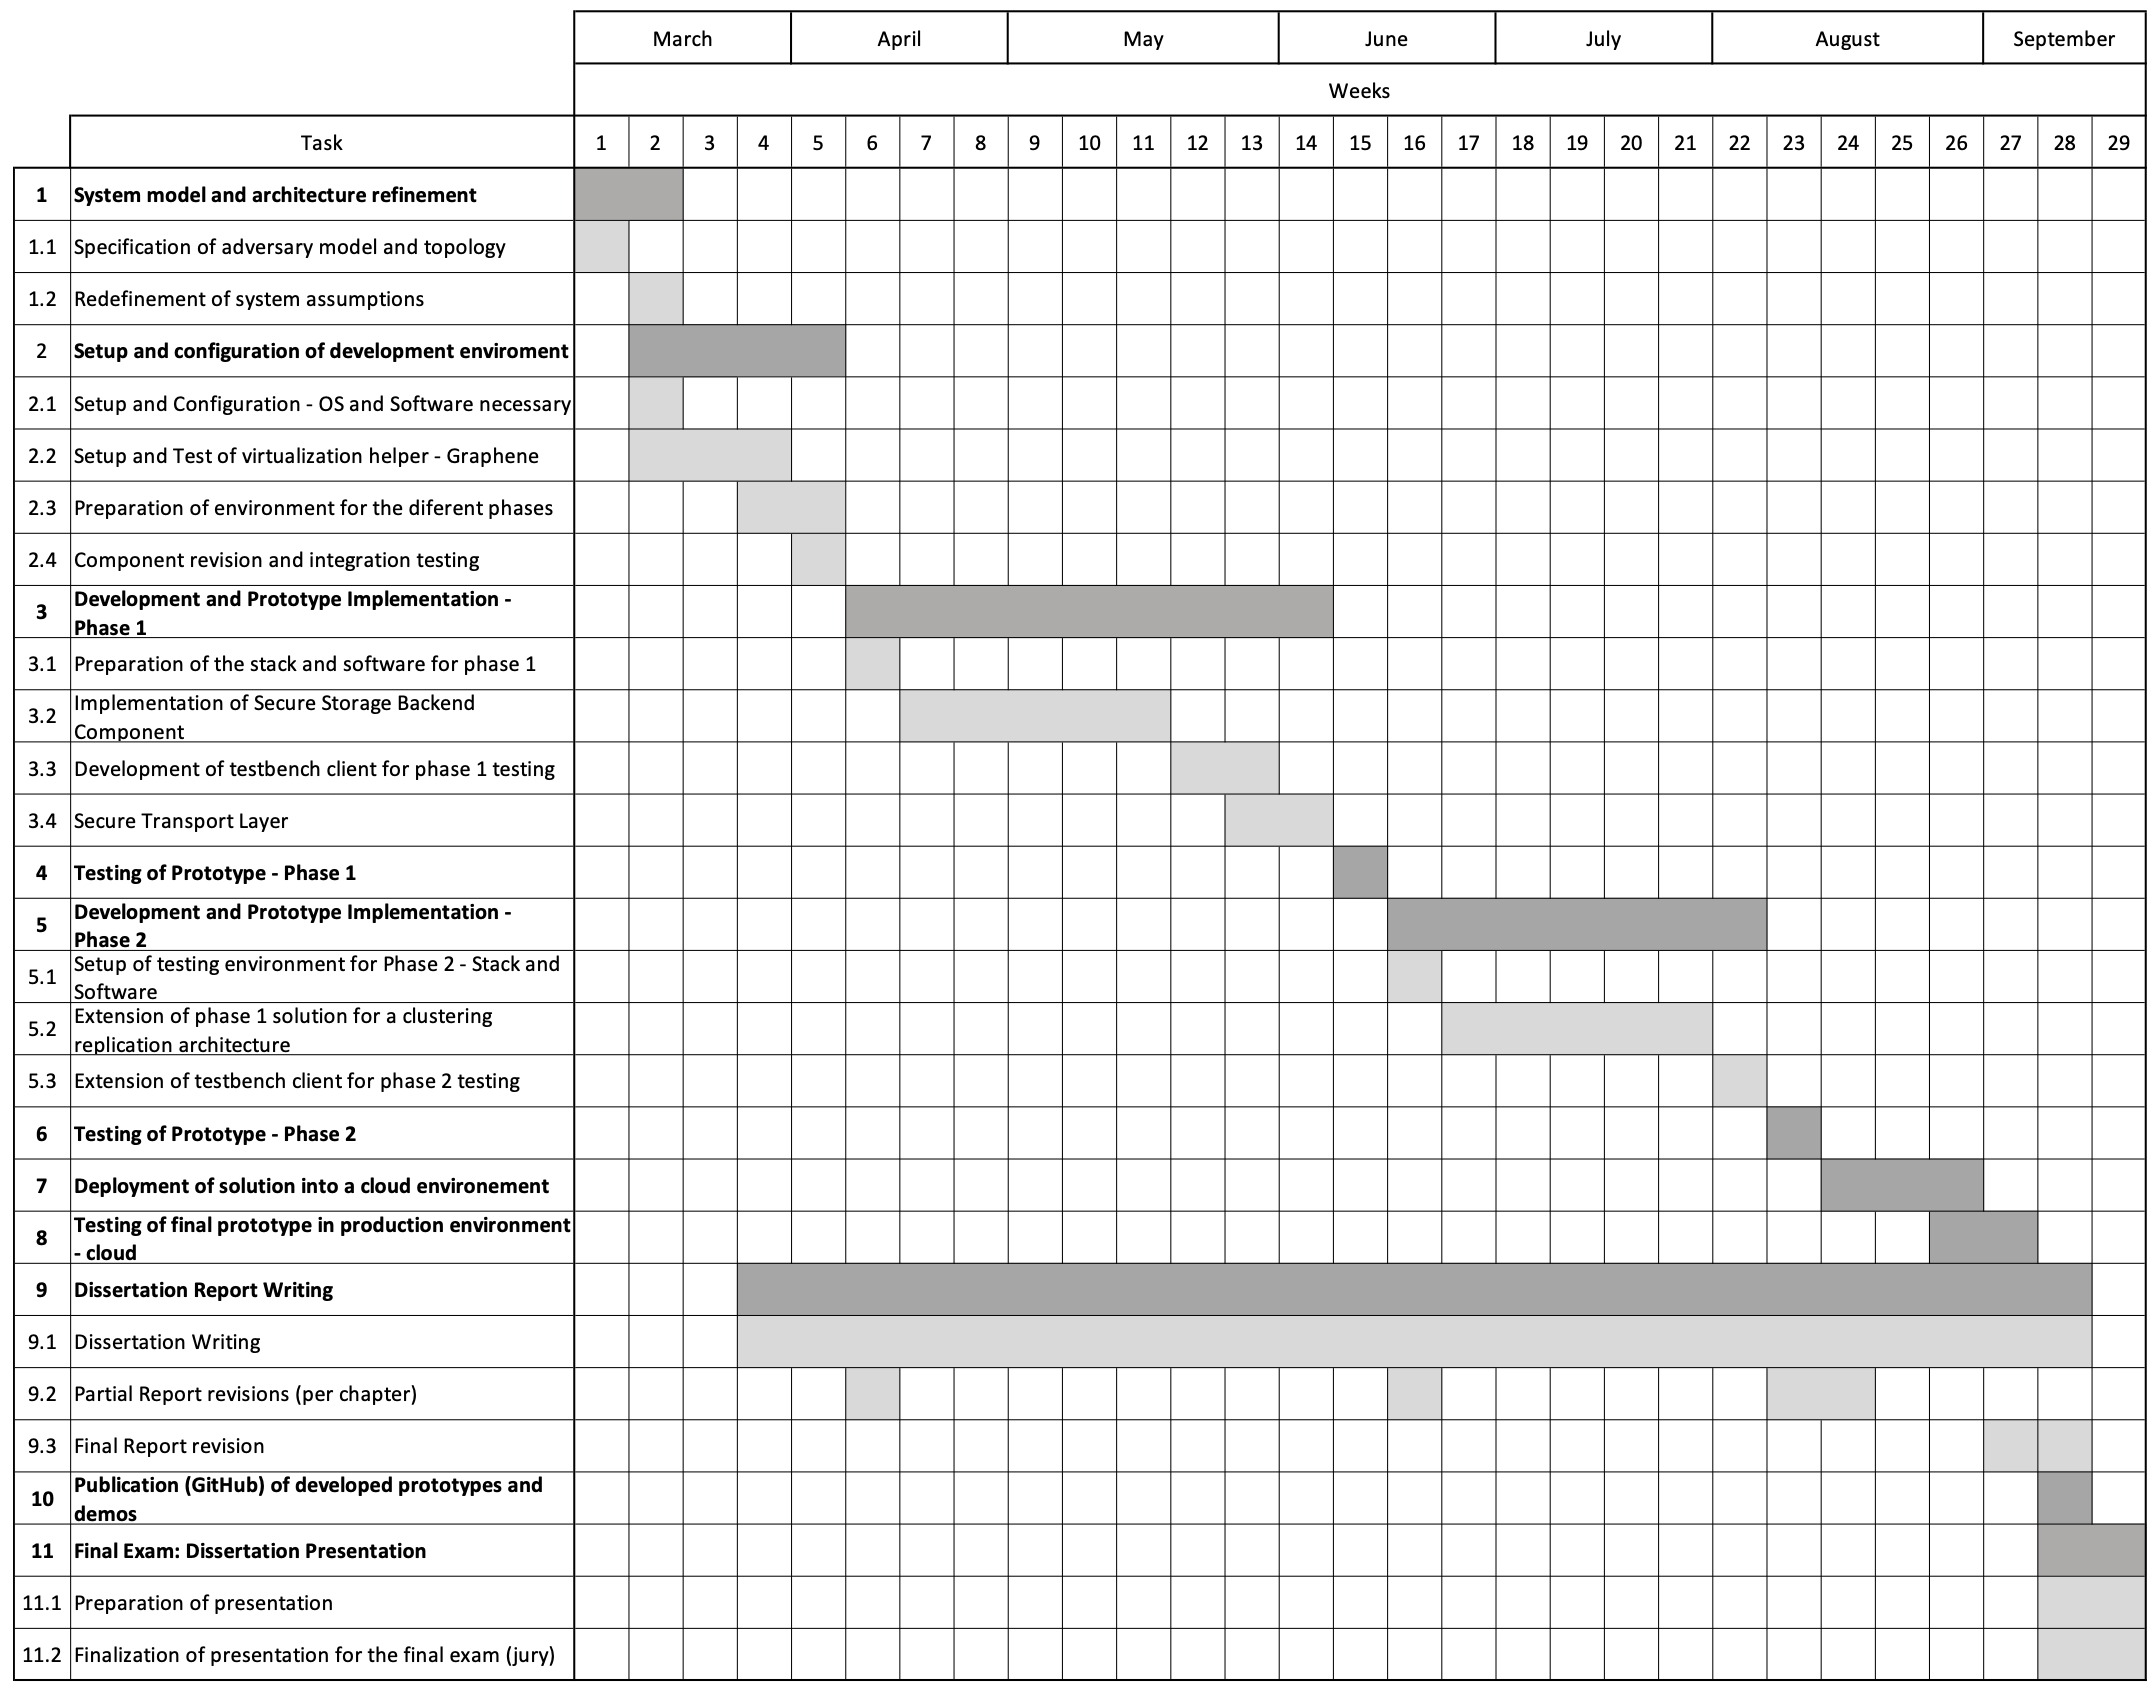
\includegraphics[angle=90, width=1.2\linewidth]{workplan}}%
	\caption{Work Plan}
	\label{fig:work_plan}
\end{figure}

\section{Work Plan Detailed Tasks}
\label{sec:workplan_details}

Figure \ref{fig:workplan_details} details the tasks shown in the work plan Gantt Chart (figure \ref{fig:work_plan}). For each task a description is available to better explain the work planned for the task, and a dependency to another task if relevant.

There are 10 main categories, called milestones that were identified, and each task will be appointed to one.

\begin{figure}[htbp]
	\centerline{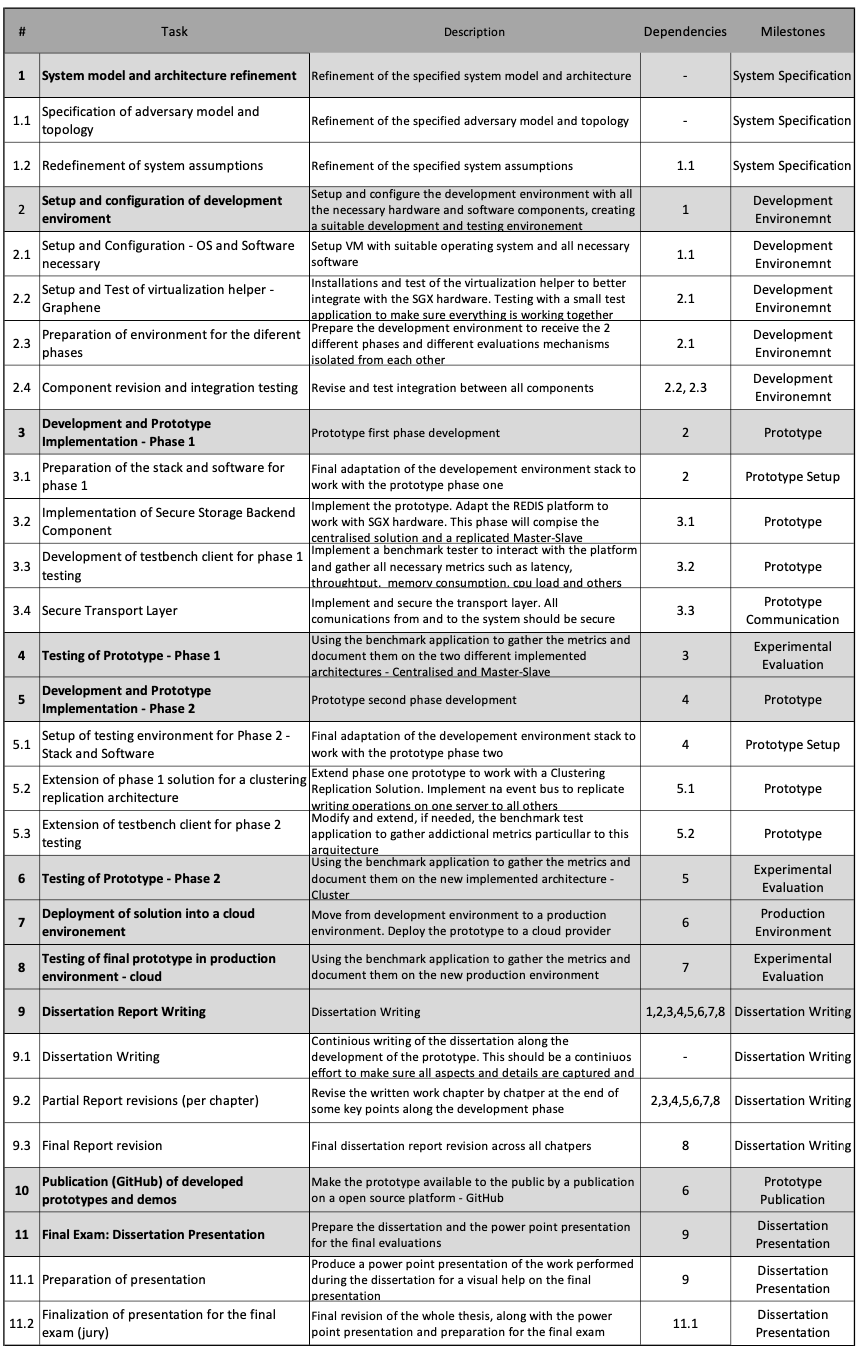
\includegraphics[width=0.99\linewidth]{workplandetails}}%
	\caption{Work Plan Details}
	\label{fig:workplan_details}
\end{figure}